\graphicspath{{sec02/images/}{sec02/code/}}
\lstset{inputpath=sec02/code/}

\begin{frame}[fragile, label=simple]{Simplest Beamer document}\relax
    \cprotect\twocolImg{
        \inputminted{latex}{sec02/code/simplest01.tex}
    }{simplest01}
    \vspace{15mm}
    % \inclassFrag{Try it! \hyperlink{style}{\beamerbutton{STYLE}} }[-1]
    \skfootnote{\ccol{label=simple} at begin frame allows to get to the frame by \ccol\hyperlink command}
\end{frame}

\begin{frame}[fragile]{Beamer document structure}{like in regular document!}\relax
    \inputminted{latex}{sec02/code/structure.tex}
    
    \skfootnote{You can also use \ccol\frame\ command}
\end{frame}

\begin{frame}[fragile]{Title page (Preamble)}{like in regular document!}\relax
    \cprotect\twocolImg{
    \inputminted[firstline=5, lastline=17]{latex}{sec02/code/title.tex}
    % \lstinputlisting[linerange={5-17}]{title.tex}
    }{title}
\end{frame}



\begin{frame}[label=style,fragile]{Built--in themes}
    % \visible<1>{\hyperlink{simple}{\beamerbutton{SIMPLE}} \\}
    \lstinline[basicstyle=\tt]|\usetheme{CambridgeUS}|\\
    \lstinline[basicstyle=\tt]|\usecolortheme{crane}|\\
    \url{https://hartwork.org/beamer-theme-matrix/}\\ \pause
    \lstinline[basicstyle=\tt]|\usefonttheme{structureitalicserif}|\\
    \url{http://deic.uab.es/~iblanes/beamer_gallery/index_by_font.html}\\ 
    \vspace{1cm}
    \inclassFrag{Google \alert{Beamer Theme Matrix} and \alert{Beamer font theme gallery}.}[-1]
\end{frame}

\begin{frame}[fragile]{TOC ({\tt AtBeginSection[]})}\relax

    \begin{columns}
        \begin{column}{0.45\textwidth}
            \expandafter\inputminted[firstline=4, lastline=8]{latex}{sec02/code/toc.tex}
        \end{column}
        \begin{column}{0.45\textwidth}
            \includegraphics[width=\textwidth, keepaspectratio,page=6]{toc.pdf}
        \end{column}
    \end{columns}
    
\end{frame}


\begin{frame}[fragile]{Frame: Columns}\relax
    \cprotect\twocolImg{
    % \lstinputlisting[linerange={8-17}]{columns.tex}
    \inputminted[firstline=8, lastline=18]{latex}{sec02/code/columns.tex}
    }{columns.pdf}
    
    (\texttt{[t]} for ``top'' align)
\end{frame}


\begin{frame}[fragile]{Colors\preMagicPage}
    \skfootnote{\wikiC{https://en.wikibooks.org/wiki/LaTeX/Colors}}
    \LaTeX\ provides several standart colors: 
    \textcolor{red}{red}, \textcolor{blue}{blue}, \textcolor{green}{green},\dots\\
    \lstinline[basicstyle=\tt]|\textcolor{red}{text}| \\
    \pause
    There many ways to define new colors, e.~g.
    \lstinline[basicstyle=\tt]|\definecolor{orange}{rgb}{1,.5,0}|\\
    \lstinline[basicstyle=\tt]|\definecolor{orange}{RGB}{255,127,0}|
\end{frame}

\begin{frame}{Colors\magicPage}
    Beamer automatically loads \alert{xcolor} package\\
    Somehow popular way to define new colors is by the following rule
    \begin{table}
    \begin{tabular}{ccc}\hline
        color           &   rgb formula             &     output  \\\hline
        red!30!blue     &   .3(1,0,0)+.7(0,0,1)     &   \textcolor{red!30!blue}{example} \\
        red!30          &   .3(1,0,0)+.7(1,1,1)     &   \textcolor{red!30!}{example}    \\ 
        red!30!blue!50!green    &   .5(red!30!blue)+.5(0,1,0)   &   \textcolor{red!30!blue!50!green}{example}   
    \end{tabular}          
    \end{table}
\end{frame}

\begin{frame}[fragile]{Blocks \& Header customisation\magicPage}
        
    \cprotect\twocolImg{
    \inputminted[firstline=7, lastline=18]{latex}{sec02/code/custom.tex}
    }{custom}
        
\end{frame}


\begin{frame}[fragile]{Appendix\magicPage}\relax
    \begin{columns}
        \begin{column}{0.45\textwidth}
            \expandafter\inputminted[firstline=8, lastline=17]{latex}{sec02/code/appendix.tex}
        \end{column}
        \begin{column}{0.45\textwidth}
            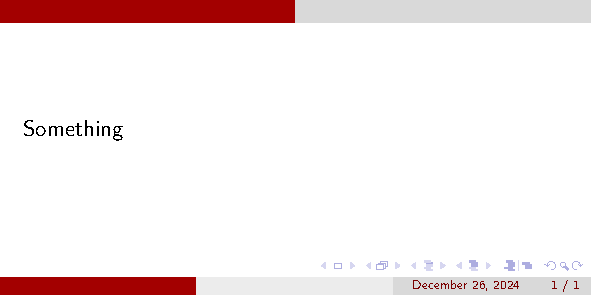
\includegraphics[width=\textwidth, keepaspectratio,page=1]{appendix}
            
            \includegraphics[width=\textwidth, keepaspectratio,page=2]{appendix}
        \end{column}
    \end{columns}
    
    (notice frame numbers!)
    
\end{frame}

\begin{frame}[fragile]{Bibliography (bibtex)\magicPage}\relax
    \cprotect\twocolImg{
    % \lstinputlisting[linerange={10-16}]{bibtex.tex}
    \inputminted[firstline=10, lastline=16]{latex}{sec02/code/bibtex.tex}
    }{bibtex.pdf}
\end{frame}

\begin{frame}[fragile]{Bibliography (simple)\magicPage}\relax
    \cprotect\twocolImg{
    % \lstinputlisting[linerange={9-21}]{bibliography.tex}
    \inputminted[firstline=9, lastline=21]{latex}{sec02/code/bibliography.tex}
    }{bibliography.pdf}
\end{frame}
